
\section{Introduction}
\begin{description}
    \item[Mobile:] Portable devices with wireless communication,
        running stand-alone or client applications.
    \item[Embedded:] An embedded system is a computer system with
        a dedicated function within a larger mechanical or electrical system.
\end{description}

Embedded systems are everywhere in smartphones, cars,\ldots Typical
characteristics is the following:
\begin{itemize}
    \item Cheap
    \item Reduced power consumption
    \item Real-time
    \item Robust
\end{itemize}

To achieve these characteristic, there need to be a tight coupling between
the hardware, the OS and the application.

\subsection{Real-Time Systems}

Real-Time Systems monitor and have an impact on the physical world via sensors
and actuators. Because of their nature, they have
requirements/constraints on timing:

\begin{description}
    \item[Hard constraint]
        \begin{itemize}
            \item Potentially severe consequences if reaction/result is produced after
                deadline.
            \item Results has no value (or even negative value) after deadline
        \end{itemize}
    \item[Firm constraint]
        \begin{itemize}
            \item Occasional miss tolerated, but degrades QoS
            \item No or little value after deadline
        \end{itemize}
    \item[Soft constraint]
        \begin{itemize}
            \item Result still has value after deadline
        \end{itemize}
\end{description}

\begin{center}
    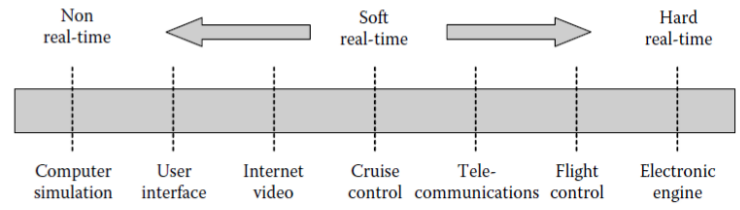
\includegraphics[width=0.7\linewidth]{img/realtime.png}
\end{center}

\subsection{Real-Time Tasks}
\begin{description}
    \item[Periodic:] Must be executed with fixed interarrival time
    \item[Sporadic:] Have known minimum interarrival time
    \item[Aperiodic:] No known interarrival time
\end{description}

\subsection{Wireless Sensor Networks}

Wireless Sensor Networks are composed of node (\textit{mote}) used for
monitoring and they communicates with each other and/or a remote server.

\subsubsection{Resource Constraint}
\begin{itemize}
    \item \textbf{Power}
        \begin{itemize}
            \item Batteries and Energy Harvesting
            \item Turn off idle devices
            \item Requires efficient OS and applications
            \item Reduce communication
        \end{itemize}

        \textit{Duty cycle} is the percentage of one period in which a
        signal or system active $\rightarrow$ isolated node will have
        high duty cycle

    \item \textbf{Bandwidth}
    \item \textbf{Memory}: just a few kBytes
    \item \textbf{CPU}: a few MHz
    \item \textbf{Data Transmission}: not enough power to reach server
        directly $\Rightarrow$ Multihop wireless Network
        \begin{itemize}
            \item Dynamic routing
            \item Self-Organizing Networks
        \end{itemize}
    \item Security: Not enough resources for sophisticated intrusion detection,
        encryption.
    \item Hardware: optimized
    \item \textbf{Reliable Data Flow}: Use 2-bit error correction and
        3-bit error detection.
        \begin{itemize}
            \item Store packet at source in circular buffer on flash 
            \item Remove data from source flash when End2End ack. (There
                is also data link ack)
        \end{itemize}
\end{itemize}

IoT = network of physical objects equipped with electronics and network
connectivity that can be sensed and controlled remotely.
